\section{Dataset and preprocessing}\label{sec:data}

\subsection{Corpus}
The corpus (\texttt{h2so4\_corpus\_final.csv}) contains 192 extracted electrode
records with 83 fields, obtained by structured extraction from published articles reporting
Ti\textsubscript{3}C\textsubscript{2}T\textsubscript{x} performance in
H\textsubscript{2}SO\textsubscript{4}. The prediction target is gravimetric capacitance
$C_g$ in F\,g\textsuperscript{-1}. Table~\ref{tab:dataset} summarises the corpus after
cleaning and Fig.~\ref{fig:dataset} shows its structure.

\subsection{Target cleaning}
A record is retained only when its capacitance is a single defensible number. Values
carrying an approximation marker (\texttt{$\sim$325}, \texttt{about 1.1}) or a mean
$\pm$ standard deviation are retained and flagged. Ranges (\texttt{300--350}) and
inequalities (\texttt{over 200}, \texttt{$<$300}) are \emph{never} collapsed to a
midpoint: 4 such rows were discarded, alongside
70 rows reporting no value.
118 rows from 40 publications survive. Two physically extreme values
(7.26 and 1609.5\,F\,g\textsuperscript{-1})
are retained and flagged rather than deleted; a sensitivity analysis excluding them from
scoring is reported in \texttt{02\_real\_only\_outlier\_sensitivity.csv}.

\subsection{Descriptor standardisation}
Thirteen descriptors were standardised by unit-aware parsing functions rather than manual
editing. Conversions are applied only where the source unit is unambiguous
($\mathrm{nm}\rightarrow\text{\AA}$, $\mathrm{mm}\rightarrow\upmu\mathrm{m}$,
$\upmu\mathrm{g\,cm^{-2}}\rightarrow\mathrm{mg\,cm^{-2}}$,
$\mathrm{V\,s^{-1}}\rightarrow\mathrm{mV\,s^{-1}}$). Incompatible bases are left
missing: a current density reported as mA\,cm\textsuperscript{-2} or
A\,cm\textsuperscript{-3} is not convertible to A\,g\textsuperscript{-1} without
information the corpus does not contain, and a mass loading given in mg or wt.\% carries no
area basis. Electrolyte molarity is parsed from the electrolyte field only; the synthesis
field also contains acid concentrations (e.g.\ wet-spinning in 98\,wt.\%
H\textsubscript{2}SO\textsubscript{4}) that are not the test electrolyte. Free-text
morphology, composition and synthesis strings are mapped to categorical families.
\texttt{synthesis\_family} collapses to a single level (LiF/HCl MILD etching~\cite{alhabeb2017}) among
the surviving rows and is therefore dropped as uninformative, leaving 12 descriptors.

\subsection{Paper grouping and leakage control}
Each row is assigned a \texttt{paper\_id} (DOI where available, else source filename; the
two are one-to-one in this corpus). Of 83 raw columns, 14 are admissible as predictors.
Excluded are volumetric and areal capacitance --- both algebraic transforms of the target
--- together with extraction-confidence and provenance metadata, free-text extraction
rationales that can quote the target value verbatim, publication identifiers, and the
\texttt{role}/\texttt{is\_primary} annotations, which are assigned with knowledge of
the measured performance. No energy- or power-density columns exist in this corpus, so the
usual $E=\tfrac{1}{2}CV^2$ leakage route is absent.

\begin{figure*}[htbp]\centering
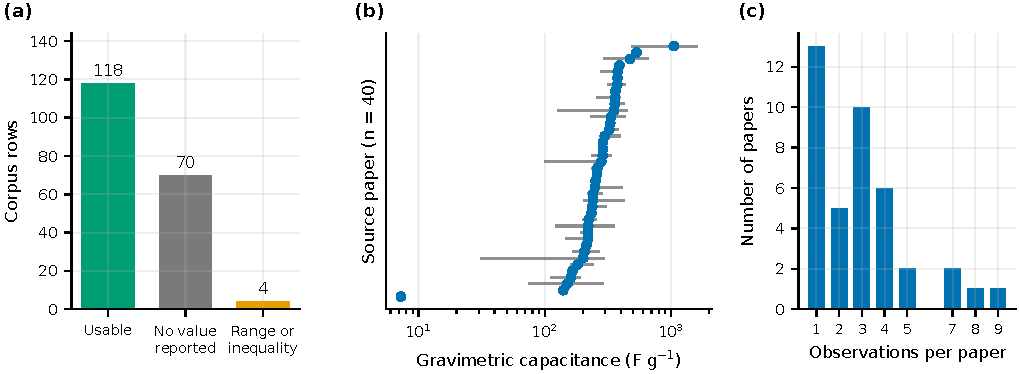
\includegraphics[width=\textwidth]{figures/fig01_dataset_structure.pdf}
\caption{Structure of the compiled corpus. (a) Disposition of the 192 raw records.
(b) Capacitance range of each of the 40 publications (bar: min--max; marker: median),
sorted by median. (c) Distribution of observations per publication. The corpus is a set of
small, tight within-paper clusters spread over a wide global range.}
\label{fig:dataset}\end{figure*}

\begin{table}[htbp]
\centering
\caption{Composition of the literature-derived H\textsubscript{2}SO\textsubscript{4} MXene corpus after target cleaning and descriptor standardisation.}
\label{tab:dataset}
\footnotesize
\begin{tabular}{lr}
\toprule
\textbf{Quantity} & \textbf{Value} \\
\midrule
Rows in the raw corpus & 192 \\
Source publications in the raw corpus & 49 \\
Rows with a usable single-valued $C_g$ & 118 \\
Publications represented after cleaning & 40 \\
Rows dropped: no value reported & 70 \\
Rows dropped: range or inequality literal & 4 \\
Approximate values retained and flagged & 2 \\
Median observations per paper & 3 \\
Maximum observations from one paper & 9 \\
Capacitance range (F\,g\textsuperscript{-1}) & 7.3--1609.5 \\
Capacitance median (F\,g\textsuperscript{-1}) & 266.5 \\
Standardised descriptors retained & 12 \\
Raw columns admissible as predictors & 14 \\
\bottomrule
\end{tabular}
\par\vspace{2pt}\begin{minipage}{\linewidth}\scriptsize Range and inequality literals (e.g.\ \texttt{300--350}, \texttt{over 200}) were discarded rather than converted to midpoints; every discarded row is logged in \texttt{01\_target\_disposition\_log.csv}.\end{minipage}
\end{table}
